\section*{Appendix}
\begin{customthm}{1}
Algorithm ${\cA^{\rm e}}$ is\\ $\big(\frac{1}{2} \sqrt{\frac{\cos \theta + 1}{2}},1\big)$-approximation for \textsc{CKP}.
\end{customthm}
\begin{proof}
 Let $S^*=\{k^*_1,...,k^*_{s^*}\}$ and $\hat S = \{k_1,...,k_s\}$ be an optimal and the  returned solution respectively, where $|S^*| = s^*$ and $|\hat S| = s$. Also let $k_{s+1}$ denote a user with $(s+1)$-th efficiency (as ordered by Eqn.~\raf{eq:ef}). For convenience, we denote $\hat d_i \triangleq d_{k_i}$, $\hat u_i \triangleq u_{k_i}$, $ d^*_j \triangleq d_{k^*_j}$, and  $ u^*_j \triangleq u_{k^*_j}$ for $i=1,...,s$ and $j=1,...,s^*$. We first sort optimal solution $S^*=\{k^*_1,...,k^*_{s^*}\}$ by efficiency in a non-increasing order as defined in Eqn.~\raf{eq:ef}, while keeping $\hat S$ order the same.
We split the analysis into two main cases:

\noindent {\bf Case (1):} $(\hat S \cup \{k_{s+1}\}) \cap S^* = \varnothing$\\
  By the greedy order (Eqn.~\raf{eq:ef}), for every $i=1,...,s+1$ we have
 \begin{align}
 \frac{\hat u_i}{|\hat d_i|} &\ge \frac{u^*_j}{|d^*_j|} \quad \text{ for all } j = 1,...,s^*.
 \end{align}
 Using the fact that $\max_i \frac{x_i}{y_i} \ge \frac{\sum_i x_i}{\sum_i y_i}$ for any positive real numbers  $x_i,y_i$; we obtain
 \begin{align}
\frac{ \hat u_i } {|\hat d_i|}&\ge \frac{\sum_{j=1}^{s^*} u^*_j}{\sum_{j = 1}^{s^*} |d^*_j|} \iff \hat u_i  \ge \frac{|\hat d_i|}{\sum_{j = 1}^{s^*} |d^*_j|} {\sum_{j=1}^{s^*} u^*_j}.
 \end{align}
 Summing up over $i=1,...,s+1$ obtains
 \begin{align}
     \sum_{i=1}^{s+1} \hat u_i &\ge {\sum_{j=1}^{s^*} u^*_j} \frac{ \sum_{i=1}^{s+1}|\hat d_i|} {\sum_{j = 1}^{s^*} |d^*_j|}. \label{eq:g.1}
 \end{align}
 In step~\ref{alg:g.max}, the algorithm returns the maximum solution. This implies
 \begin{align}
 \max\{u(S_1), u(S_2)\} &\ge \frac{1}{2} \big( \sum_{i=1}^{s} \hat u_i + u_{\max}\big) \ge \frac{1}{2} \sum_{i=1}^{s+1} \hat u_i \nonumber\\
 & \ge \frac{1}{2}\cdot \frac{ \sum_{i=1}^{s+1}|\hat d_i|} {\sum_{j = 1}^{s^*} |d^*_j|} \OPT, \label{eq:g.2}
 \end{align}
 where $u_{\max} \triangleq \max_{k\in \cN} u_k$, and Eqn.~\raf{eq:g.2} follows by Eqn.~\raf{eq:g.1}. Finally, we bound $\frac{ \sum_{i=1}^{s+1}|\hat d_i|} {\sum_{j = 1}^{s^*} |d^*_j|}$ from below.  Since $\theta$ is at most $\frac{\pi}{2}$, and $|\sum_{i=1}^{s+1} \hat d_i | \ge C \ge |\sum_{j=1}^{s^*}  d^*_j$, we can apply Lemma~\ref{lem:tb} below and obtain: 
\begin{equation} 
\frac{ \sum_{i=1}^{s+1}|\hat d_i|} {\sum_{j = 1}^{s^*} |d^*_j|} \ge \frac{\big|\sum_{j=1}^{s^*} d^*_j \big|}{\sum_{j = 1}^{s^*} |d^*_j|}\ge \sqrt{\frac{\cos \theta + 1}{2}}. \label{eq:g.3}
 \end{equation}
 (See figure~\ref{fig:greedy} for a pictorial intuition).
\begin{figure}[!ht]
	\begin{center}
		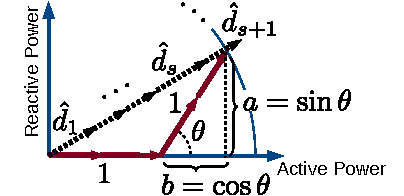
\includegraphics[scale=0.8]{fig/fig-greedy.pdf}
	\end{center}
\caption{The figure depicts an extreme case where the ratio  $\frac{\sum_{i=1}^{s+1} |\hat d_i|}{\sum_{j = 1}^{s^*} |d^*_j|}$ is minimal. The dotted arrows represent solution $\hat S \cup \{k_{s+1}\}$ (which is in-feasible), whereas the red arrows are  optimal solution $S^*$. One can show that the two optimal sides are equal (in the extreme case). By rescaling the triangle such that each of the two optimal sides are equal to 1, $\sum_{i=1}^{s+1}|\hat d_i| \ge \sqrt{(1+\cos \theta)^2 + \sin^2 \theta} = \sqrt{2 + 2\cos \theta}$. Therefore $\frac{\sum_{i=1}^{s+1} |\hat d_i|}{\sum_{j = 1}^s |d^*_j|} \ge \frac{\sqrt{2 + 2\cos \theta}}{2}=\sqrt{\frac{\cos \theta + 1}{2}}$.}
	\label{fig:greedy}
\end{figure}  
  Combining Eqns.\raf{eq:g.2}-\raf{eq:g.3} gives
 \begin{equation}
  \max\{u(S_1), u(S_2)\} \ge \frac{1}{2} \sqrt{\frac{\cos \theta + 1}{2}} \cdot \OPT. \label{eq:g.3.5}
 \end{equation}
 
\noindent {\bf Case (2):} $(\hat S \cup \{k_{s+1}\}) \cap S^* \neq \varnothing$\\
For convenience we use $i \in  S\cap S^* $, $i \in  S\backslash S^* $, $j \in S^*\backslash  S $ to indicate $k_i \in  (\hat S \cup {k_{s+1}} )\cap S^*$,  $k_i \in  (\hat S \cup {k_{s+1}} )\backslash S^*$, and  $k^*_j \in  S^*\backslash (\hat S \cup {k_{s+1}} )$ respectively.
   By the greedy order (Eqn.~\raf{eq:ef}), for every $i= S\backslash S^*$ we have
$\frac{\hat u_i}{|\hat d_i|}\ge \frac{u^*_j}{|d^*_j|} \quad \text{ for all } j \in S^*\backslash  S$.
 This implies that,
 \begin{equation}
  \frac{ \sum_{i\in  S \backslash S^*} \hat u_i}{ \sum_{i\in  S \backslash S^* }|\hat d_i|}  \ge \frac{\sum_{j \in S^*\backslash  S} u^*_j} {\sum_{j \in S^*\backslash  S} |d^*_j|}. \label{eq:g.4}
 \end{equation}

Next, if $\sum_{i\in  S \backslash S^*}  |\hat d_i| \ge \sum_{j \in S^*\backslash  S} |d^*_j|$ (by Eqn.\raf{eq:g.4}, it implies $\sum_{i\in  S \backslash S^*} \hat u_i \ge \sum_{j \in S^*\backslash  S} u^*_j$) then $\sum_{i=1}^{s+1} \hat u_i \ge \OPT$. Therefore, w.l.o.g., we assume   $\sum_{i\in  S \backslash S^*}  |\hat d_i| < \sum_{j \in S^*\backslash  S} |d^*_j|$
 
 By Lemma~\ref{lem:frac}
 \begin{align}
& \frac{\sum_{i\in  S  \cup S^*} \hat u_i +  \sum_{i\in  S \backslash S^*} \hat u_i}{ \sum_{i\in  S  \cup S^*} |\hat d_i| + \sum_{i\in  S \backslash S^* }|\hat d_i|}  \ge \frac{\sum_{i\in  S  \cup S^*} \hat u_i \sum_{j \in S^*\backslash  S} u^*_j} {\sum_{i\in  S  \cup S^*} |\hat d_i|  + \sum_{j \in S^*\backslash  S} |d^*_j|}\\
 & \sum_{i=1}^{s+1} \hat u_i \ge  \frac{ \sum_{i=1}^{s+1}|\hat d_i|} {\sum_{j = 1}^{s^*} |d^*_j|}\cdot  \OPT \ge \sqrt{\frac{\cos \theta + 1}{2}} \cdot \OPT \label{eq:g.5},
 \end{align}
 where Eqn.~\raf{eq:g.5} follow from Eqn.~\raf{eq:g.3}. The rest is similar to Eqn.~\raf{eq:g.2}-\raf{eq:g.3.5}.
 
 
 Finally, we mention that the algorithm always obtains a feasible solution (by  step~\ref{alg:g.feas} condition), the algorithm is ${\cA^{\rm e}}$ is\\ $\big(\frac{1}{2\sqrt 2} \sqrt{\cos \theta + 1},1\big)$-approximation.
\end{proof}
\


\begin{lemma}
\label{lem:tb}
Given a set of 2D vectors $\{d_i \in \RR^2\}_{i=1}^n$
$$ \frac{\sum_{i=1}^n |d_i| }{\big| \sum_{i =1}^n d_i \big|} \le \sqrt{\frac{2}{\cos \theta + 1}},$$
where $\theta$ is the maximum angle between any pair of vectors and $0 \le \theta \le \frac{\pi}{2}$.
\end{lemma}
\begin{proof}
We proof $\frac{(\sum_{i=1}^n |d_i| )^2}{|\sum_{i=1}^n d_i |^2} \le \frac{\cos + 1}{2}$  by induction. First, we expand  the L.H.S.
\begin{align}
&\frac{  \sum_{i=1}^n |d_i|^2 +  2\sum_{1\le i < j \le n} |d_i| \cdot |d_j|  } { \sum_{i =1}^n |d_i|^2 +  2\sum_{1\le i < j \le n} |d_i| \cdot |d_j| (\sin \theta_i \sin \theta_j + \cos \theta_i \cos \theta_j)}\nonumber\\
&=\frac{ \sum_{i=1}^n |d_i|^2 +  2\sum_{1\le i < j \le n} |d_i| \cdot |d_j|  } { \sum_{i=1}^n |d_i|^2 +  2\sum_{1\le i < j \le n} |d_i| \cdot |d_j| \cos (\theta_i - \theta_j)}, \label{eq:ind}
\end{align}
where $\theta_i$ is the angle that $d_i$ makes with the $x$ axis.


Consider the base case: $|S|= 2$. Eqn.~\raf{eq:ind} is
\begin{align}
 \frac{|d_1|^2 +|d_2|^2 + 2 |d_1|\cdot |d_2|}{|d_1|^2 +|d_2|^2 + 2 |d_1|\cdot |d_2| \cos(\theta)} = f(x),
\end{align}
where $ f(x) \triangleq \frac{1+x^2+2x}{1+x^2+2x\cos \theta}$ and $x=\frac{|d_2|}{|d_1|}$. The first derivative $f'(x) = \frac{(1+x^2+2x \cos \theta )(2x + 2) - 1+x^2 + 2x)(2x + 2 \cos \theta)}{(1 + x^2 + 2x \cos \theta )^2}$ is zero only when $x=1$. Hence, $f(1)$ is an extreminum point.  We compare $f(1)$ with $f(x)$ at the  boundaries $x\in \{0,\infty\}$: $f(1) = \frac{2}{\cos \theta + 1} \ge f(0) = \lim_{x \to \infty} f(x) = 1$. Therefore $f(x)$ has a global maximum of $\frac{2}{\cos \theta  + 1}$.

Next we proceed to the inductive step. We assume $\frac{\sum_{i=1}^{r-1} |d_i| }{\big| \sum_{i=1}^{r-1} d_i \big|} \le \sqrt{\frac{2}{\cos \theta + 1}}$ where $r \in \{1,\ldots, n\}$. W.L.O.G., assume $\theta_1\ge\theta_3\ge \cdots \ge \theta_n \ge \theta_2$. Rewrite Eqn.~\raf{eq:ind}:
\begin{equation}
 \frac{ ( \sum_{i=1}^r |d_i|)^2 } { \displaystyle \sum_{i=1}^r |d_i|^2 + 2 \smashoperator{\sum_{1\le i<j<r}} |d_i|  |d_j| \cos (\theta_i - \theta_j) +  2 |d_r| \smashoperator{\sum_{1\le i<r}} |d_i|  \cos (\theta_i - \theta_r)}. \label{eq:den}
\end{equation}
Let $g(\theta_r)$ be the denominator of Eqn.~\raf{eq:den}. We take the  second derivative of $g(\theta_r)$:
$$g''(\theta_r) = -2 |d_r| \sum_{1 \le i < r} |d_i| \cos(\theta_i - \theta_r).$$ Notice that $\cos(\theta_i - \theta_r) \ge 0$, therefore the second derivative is always negative. This indicates that all local exterma in $[0,\theta_{r-1}]$ of $g(\theta_n)$ are local maxima. Hence, the minimum occur at the boundaries:
\begin{equation}
\min_{\theta_r \in [0,\theta_{r-1}]}  g(\theta_r) \in \{g(0), g(\theta_{r-1})\}
\end{equation}
If $\theta_r \in \{0,\theta_r\}$ there must exist at least a pair of vectors in $\{d_i\}_{i=1}^r$ with the same angle. Combining these two vectors into one, we can obtain an instance with $r-1$ vectors. Hence, by the inductive hypothesis, the same bound holds up to $r$ vectors.
\end{proof}
\

\begin{lemma} 
\label{lem:frac}
Given $\frac{x}{y} \ge \frac{a_1}{b_1} \ge \frac{a_2}{b_2}$ such that  $b_1 < b_2$
$$ \frac{x+a_1}{y+b_1} \ge \frac{x+a_2}{y + b_2},$$
where $x,y,a_1,a_2,b_1$ and $b_2$ are positive real numbers.
 \end{lemma}
 \begin{proof}
 We show $\frac{x+a_1}{y+b_1} - \frac{x+a_2}{y + b_2} \ge 0 $.
 \begin{align}
 &\frac{x+a_1}{y+b_1} - \frac{x+a_2}{y + b_2}  = \frac{x(b_2 - b_1) + y(a_1 - a_2) + a_1 b_2 - a_2 b_1 }{(y+b_1)(y+b_2)} \nonumber\\
 &\ge  \frac{x(b_2 - b_1) + y(a_1 - a_2) }{(y+b_1)(y+b_2)}
 \end{align}
 We complete the proof  showing $x(b_2 - b_1) \ge   - y(a_1 - a_2)$.
 \begin{align}
 \frac{x}{y} + \frac{a_1 - a_2}{b_2 - b_1} \ge   \frac{a_1}{b_1} + \frac{a_1 - a_2}{b_2 - b_1} = \frac{a_1 b_2 - a_2 b_1}{b_1 ( b_2 - b_1)} \ge 0
 \end{align}
 \end{proof}
 
